\documentclass[conference]{IEEEtran}
\IEEEoverridecommandlockouts
% The preceding line is only needed to identify funding in the first footnote. If that is unneeded, please comment it out.
\usepackage{cite}
\usepackage{amsmath,amssymb,amsfonts}
\usepackage{algorithmic}
\usepackage{graphicx}
\usepackage{textcomp}
\usepackage{xcolor}
\def\BibTeX{{\rm B\kern-.05em{\sc i\kern-.025em b}\kern-.08em
    T\kern-.1667em\lower.7ex\hbox{E}\kern-.125emX}}
\begin{document}

\title{Predicting Cancer Malignancy with Limited Data\\
{\footnotesize \textsuperscript{*}Note: A Project Presented as part of the requirements for BIOF 509: Applied Machine Learning}
}

\author{\IEEEauthorblockN{Evaristus Mbanefo}
\IEEEauthorblockA{\textit{Laboratory of Immunology} \\
\textit{NEI, NIH}\\
Bethesda, United States \\
evambanefo@yahoo.com }

}

\maketitle

\begin{abstract}
Machine Learning has become very pivotal to Medicine. There are several tools that aid quick diagnosis and monitoring of treatment and prognosis. The entrance of machine learning has revolutionalized this approach. There is now a data driven approach that can predict presence or severity of disease based on data collected overtime from previous patients. This approach can even include data on drug treatment with good prognosis to direct best treatment. Using data collected from breast cancer patients, this tool is able to not only generate a model to predict breast cancer malignancy at over 0.95 accuracy. Above all, although this model used 31 variables, we show that the same result can be obtained at 0.92 accuracy using only 4 of the variables. This is important in situations where there is missing data or the use of equipment that do not collect all 31 variables for data collection. 
\end{abstract}

\begin{IEEEkeywords}
component, formatting, style, styling, insert
\end{IEEEkeywords}

\section{Introduction}
Machine Learning has come to stay and is becoming increasingly important in Medical practice. Machine learning tools take advantage of data to generate tools that aid quick diagnosis and monitoring of treatment and prognosis (Mostavi et al, 2015, Guo et al, 2015). In this era of personalized medicine (Haendel, 2018), this has become even more important. The entrance of machine learning has revolutionalized all aspects of medicine from social medicine up to neurosurgery, its application can be found in all aspects of health care. 

There is increasingly data driven approaches that can be adopted (LeeCun et al, 2015) to take advantage of otherwise stored records to predict presence or severity of disease based on data collected overtime from previous patients. This approach can even include data on drug treatment with good prognosis to direct best treatment. Some studies have applied ML algorithms like convolutional neural networks for cancer prediction (Mostavi et al, 2015, De et al, 2013, Lyu et al, 2018). 

Here, we use data collected from breast cancer patients, this tool is able to not only generate a model to predict breast cancer malignancy at over 0.95 accuracy. Above all, although this model used 31 variables, we show that the same result can be obtained at 0.92 accuracy using only 4 of the variables. This is important in situations where there is missing data or the use of equipment that do not collect all 31 variables for data collection. 

\section{Method}

\subsection{The data}

Machine learning takes advantage of otherwise stagnant data or information in addition to continuous data collection. This results in enormous conservation of resources which can be focused on other aspect of the health care. The data utilized in this project is extracted from breast cancer images. Several features were extracted from the slides and converted into .csv file for easy processing. The data is available freely online at scikit-learn.

The variables are: 
'mean radius', 'mean texture', 'mean perimeter', 'mean area',
        'mean smoothness', 'mean compactness', 'mean concavity',
        'mean concave points', 'mean symmetry', 'mean fractal dimension',
        'radius error', 'texture error', 'perimeter error', 'area error',
        'smoothness error', 'compactness error', 'concavity error',
        'concave points error', 'symmetry error',
        'fractal dimension error', 'worst radius', 'worst texture',
        'worst perimeter', 'worst area', 'worst smoothness',
        'worst compactness', 'worst concavity', 'worst concave points',
        'worst symmetry', 'worst fractal dimension'. The classification were either Malignant or Benign.

\section{Data Exploration}
We first explored the data, converting into DtaFrame for easy preprocessing. For preprocessing, we used pandas, numpy, seaborn and matplotlib.pyplot libraries. After examining the data and exploring missing data, we confirmed the integrity of the data and visualised the head and tail. We plotted histogram of the two classes, in addition to the combined data. This enabled us to use the distribution of the data to decipher the variables that impacted the prediction more robustly.

The most significant parameters were mean radius, mean perimeter, mean area and mean concavity (Fig 1 - Fig 4) which were very efficient in distinguishing between the malignant and benign cases. We also show examples of variables that showed poor differential between the cancer severity categories, namely: mean fractal dimension, mean symmetry, mean smoothness and mean texture.


\begin{figure}[htbp]
\centerline{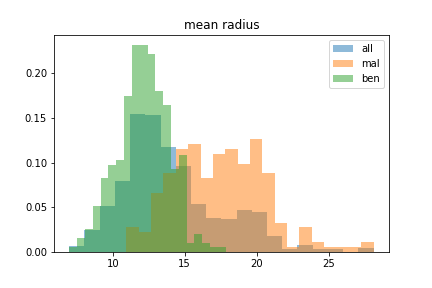
\includegraphics [width = 7cm] {mean radius.png}}
\caption{Mean Radius (good correlation)}
\label{fig}
\end{figure}
\begin{figure}[htbp]
\centerline{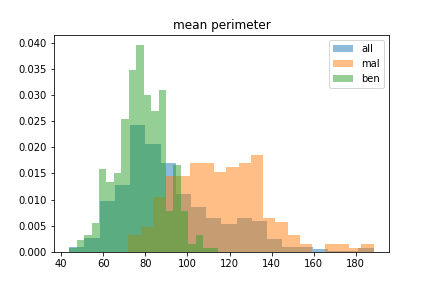
\includegraphics [width = 7cm] {mean perimeter.png}}
\caption{Mean Perimeter (good correlation)}
\label{fig}
\end{figure}
\begin{figure}[htbp]
\centerline{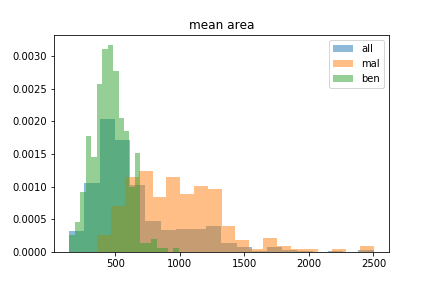
\includegraphics [width = 7cm] {mean area.png}}
\caption{Mean Area (good correlation)}
\label{fig}
\end{figure}
\begin{figure}[htbp]
\centerline{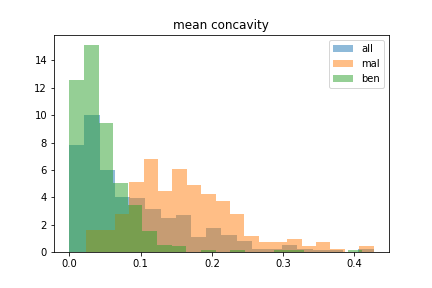
\includegraphics [width = 7cm] {mean concavity.png}}
\caption{Mean Concavity (good correlation)}
\label{fig}
\end{figure}



\begin{figure}[htbp]
\centerline{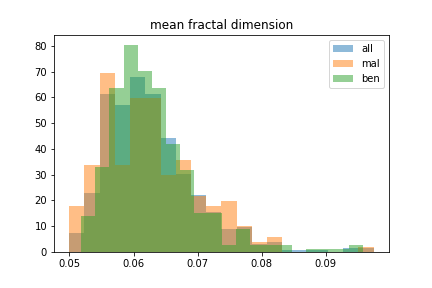
\includegraphics [width = 7cm] {mean fractal dimension.png}}
\caption{Mean Fractal Dimension (poor correlation)}
\label{fig}
\end{figure}
\begin{figure}[htbp]
\centerline{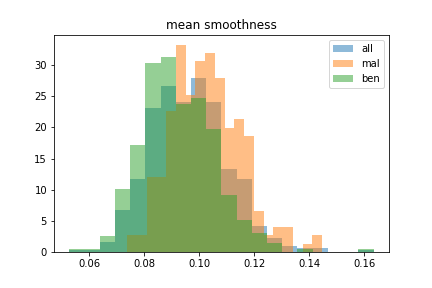
\includegraphics [width = 7cm] {mean smoothness.png}}
\caption{Mean Smoothness (poor correlation)}
\label{fig}
\end{figure}
\begin{figure}[htbp]
\centerline{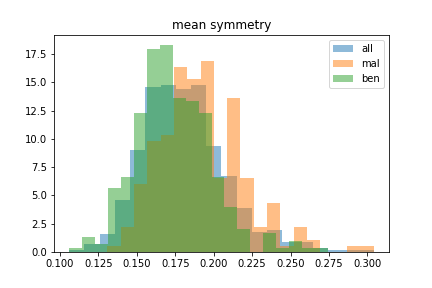
\includegraphics [width = 7cm] {mean symmetry.png}}
\caption{Mean Symmetry (poor correlation)}
\label{fig}
\end{figure}
\begin{figure}[htbp]
\centerline{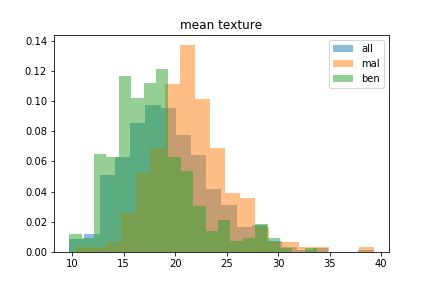
\includegraphics [width = 7cm] {mean texture.png}}
\caption{Mean Texture (poor correlation)}
\label{fig}
\end{figure}


\section{Modeling}
\subsection{Objective}\label{AA}
Some of the variables available for a predictive model of cancer were of little value for the model. For instance, while radius, perimeter, area, concavity and concave point showed appreciable potential to differentiate breast cancer severity, the other variables were of less value in any predictive model from this dataset. 

Moreso, the distribution of observations within the useful variables showed significant overlap between benign and malignant disease. We propose to generate an alternative predictive model using these variables with good correlations and compare the performance to model built using all the variables. We will then make a program that accepts few inputs from user to provide a predicition of cancer severity..

\subsection{Label Encoding and Splitting}
We used LabelEncoder and train test split functions in sklearn preprocessing and sklearn model selection, respectivly to randomly assign data to either training sets or testing set. The training set will be used for the training while the testing set will be used for validation.

\subsection{Scaling and Standardization}
We used the StandardScaler function also from sklearn package to scale both the x and y data in preparation for learning. The code blocks are in the Final project codes in github.

\subsection{Model Selection}
For the model selection, we imported both the Linear LogisticRegression, Support Vector Matrix and the k-means nearest neighbour models. The models were applied with optional parameters and thenn model fitting was performed, ready for prediction. An example of the code block can be seen below:
 
\begin{equation}
from sklearn.neighbors import KNeighborsClassifier
\end{equation}
\begin{equation}
BC_classifier2 = KNeighborsClassifier (...)
\end{equation}
\begin{equation}
BC_classifier2.fit(Variables_train, Diagnosis_train)
\end{equation}


\subsection{Prediction and Confusion Matrix}
Next we used the test dataset to perform predictions, exported the result of the prediction to a DataFrame before calculating teh confudion matrix. Confusion matrix will use th enumber of correct and incorrect predictions to calculate the accuracy of the model. Based on our model and subsequent prediction, accuracy of over 0.958 our of 1 was observed. The k-means model returned o.951 accuracy.


		Correctly predicted malignant: 50
		Incorrectly predicted malignant: 3
		Correctly predicted benign: 87
		Incorrectly predicted benign: 3
		Total of correct prediction: 137
		Total of incorrect prediction: 6
		Performance: 95.8041958041958


\subsection{Model and Prediction based on fewer variables}
We found earlier that a few variables impacted the model more than others. We attempted to repeat the prediction using only these four variables. Interestingly, the model still returned up to 0.9231 accuracy. 

\begin{figure}[htbp]
\centerline{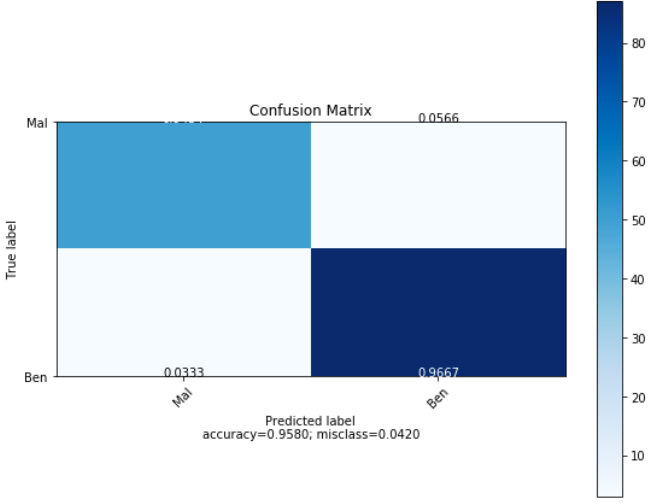
\includegraphics [width = 7cm] {cm1.png}}
\caption{Confusion Matrix for Model with 4 variables (0.958 accuracy)}
\label{fig}
\end{figure}
\begin{figure}[htbp]
\centerline{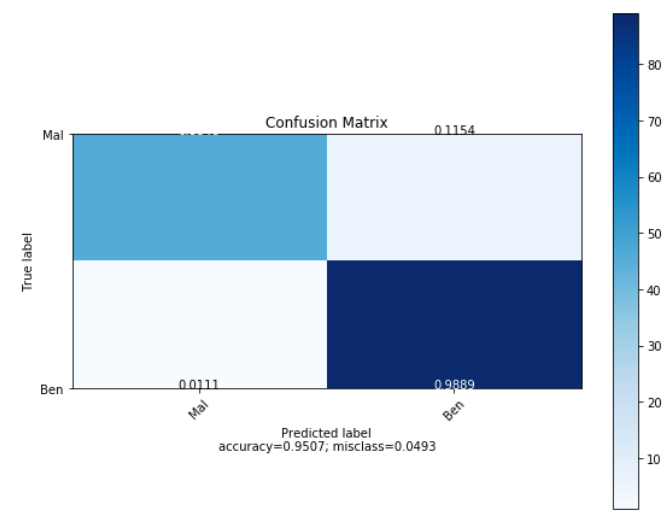
\includegraphics [width = 7cm] {cm2.png}}
\caption{Confusion Matrix for Model with K means (0.9507 accuracy)}
\label{fig}
\end{figure}
\begin{figure}[htbp]
\centerline{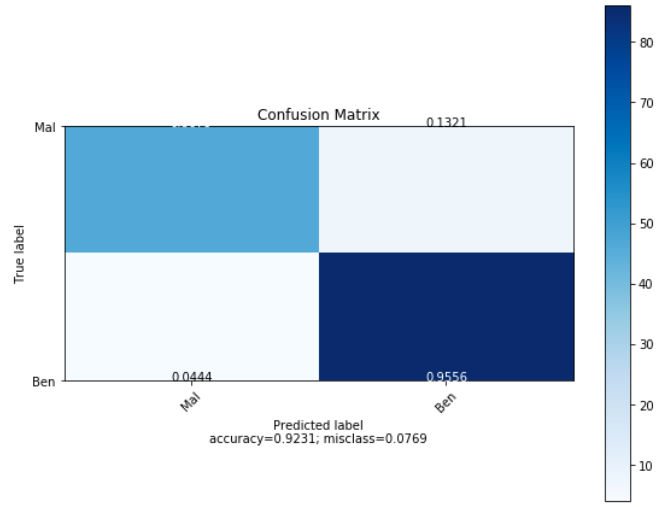
\includegraphics [width = 7cm] {cm4.png}}
\caption{Confusion Matrix for Model with 4 variables (0.9231 accuracy)}
\label{fig}
\end{figure}


\section{User Interface (Future prospect and Conclusiom)}
We envisage future application of this model in the clinic, including in the case of incomplete data. Our tool will prompt user to enter values for variables starting with the key variables and will readily predict severity based on as few as the 4 major variables: mean radius, mean parameter, mean area, and mean concavity.

\begin{figure}[htbp]
\centerline{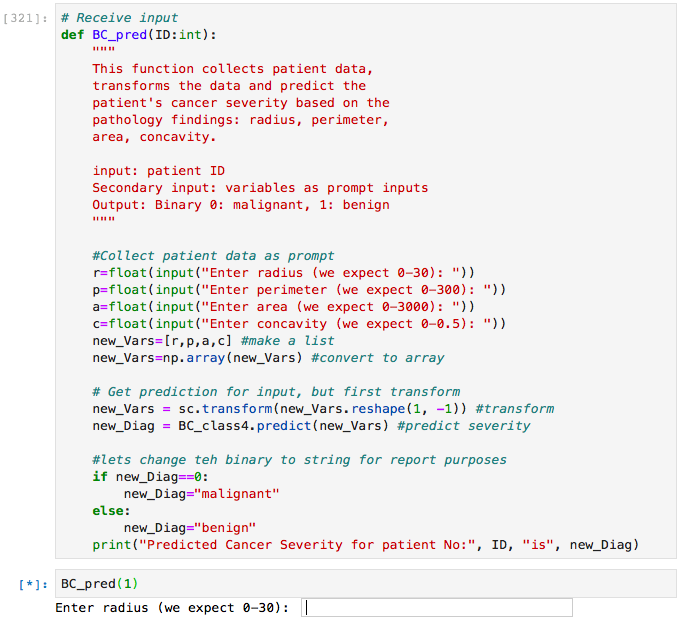
\includegraphics [width = 9cm] {newtool.png}}
\caption{User Interface}
\label{fig}
\end{figure}

\section{Conclusiom)}
Our work will contribute to quick diagnosis and classification of cancer. Such tool will still be useful, even in the situation of missing data since our algorithm did not need the 30 variables for accuracy. The user interface is a work in progress and can be further developed with other intuitive features to both make it amenable and accurate for clinical application. 



\section*{Acknowledgment}

Grateful to Dr James Anibal, Christina T and FAES.



\begin{thebibliography}{00}

\bibitem{b1} Milad Mostavi, Yu-Chiao Chiu, Yufei Huang and Yidong Chen, ``Convolutional neural network models for cancer type prediction based on gene expression,'' (2015).  BMC Medical Genomics, 2020; 13 (Suppl 5): 44 DOI: 10.1186/s12920-020-0677-2

\bibitem{b2} Peng Guo; Koyel Banerjee; R. Joe Stanley; Rodney Long; Sameer Antani; George Thoma; Rosemary Zuna; Shelliane R. Frazier; Randy H. Moss; William V. Stoecker, Nuclei-Based Features for Uterine Cervical Cancer Histology Image Analysis With Fusion-Based Classification. IEEE Journal of Biomedical and Health Informatics (Vol 20, issue 6 pp. 1595-1607) DOI: 10.1109/JBHI.2015.2483318

\bibitem{b3} Haendel MA, Chute CG, Robinson PN. Classification, ontology, and precision medicine. N Engl J Med. 2018;379(15):1452?62.

\bibitem{b4} S. De, R. J. Stanley, C. Lu, R. Long, S. Antani, G. Thoma, et al., "A fusion-based approach for uterine cervical cancer histology image classification", Comput. Med. Imag. Graph., vol. 37, pp. 475-487, 2013.

\bibitem{b5} LeCun Y, Bengio Y, Hinton G. Deep learning. Nature. 2015;521(7553):436?44.

\bibitem{b6} Lyu B, Haque A. Deep learning based tumor type classification using gene expression data. In: Proceedings of the 2018 ACM International Conference on Bioinformatics, Computational Biology, and Health Informatics: ACM; 2018. p. 89?96.

\end{thebibliography}{00}
\vspace{12pt}


\end{document}
